\capitulo{5}{Aspectos relevantes del desarrollo del proyecto}



\section{Conceptos usados aprendidos en la Universidad}

\subsection{Programación en lenguaje Python}
Python es un lenguaje que ha sido utilizado en diversas asignaturas a lo largo de la carrera como por ejemplo Algoritmia, Sistemas Inteligentes, Gestión de la Información o Computación Neuronal y Evolutiva. En cada una de estas asignaturas han sido enseñadas diferentes librerías como por ejemplo Matplotlib la cual es fundamental para mostrar los resultados de este trabajo.

Se agradecen también las horas de practicas de estas asignaturas las cuales han sido muy importantes a la hora de conseguir cierta soltura para programar en este lenguaje.

\subsection{Conocimientos sobre intérpretes y compiladores}
La forma en que un compilador trata la información para transformarla y el uso que tiene el intérprete ha sido un tema central que se nos ha enseñado en la asignatura de Procesadores del lenguaje. 

\subsection{Programación eficiente}
En asignaturas como Programación y Metodología de la programación, se han enseñado maneras de llevar a cabo una programación que se han llevado a cabo en este desarrollo.

\subsection{Gestión del desarrollo}
Hay también que nombrar a la asignatura Gestión de Proyectos, donde se aprendió sobre la metodología Kanban utilizada en este proyecto y también sobre como utilizar la aplicación Github. 

\section{Transcurso del desarrollo}

El planteamiento inicial del proyecto era crear una herramienta para medir la eficiencia del código Python, en base a los ciclos de reloj y el espacio en memoria que este ocupa. Al ser este un planteamiento previo al inicio del desarrollo, este ha ido dando algunos cambios según nuevos requisitos han ido surgiendo o restricciones con las que no habíamos contado han ido apareciendo. En este apartado se intentara contar como han surgido esos cambios inesperados y como han afectado este al desarrollo del proyecto.\\

\subsection{El intérprete}

En primer lugar, la base por donde se partió el proyecto fue el intérprete. Se buscó un intérprete capaz de satisfacer las necesidades que se plantearon. En esta etapa surgieron varias propuestas, pero tras algunas puestas en común, se llegó a la conclusión de que el intérprete ByteRun era la mejor idea para hacer un primer intento.\\

\subsubsection{Requisitos que cumple}
ByteRun al final fue el intérprete elegido porque nos proporcionaba una serie de requisitos que encajaban a la perfección con lo que teníamos planeado previamente. He aquí alguno de esos requisitos:\\

\begin{itemize}
	\item Estaba desarrollado en Python: Al ser Python un lenguaje conocido y que ha sido impartido en la Universidad, era preferible que estuviese hecho en un lenguaje que ya tuviésemos conocimientos previos. Además que un intérprete de Python hecho en Python nos parecía que tenía un cierto atractivo.
	\item Los autores de este interprete contaban con una buena documentación sobre su funcionamiento\cite{ByteRunGithub}, lo cual nos venía como anillo al dedo, para así entender mejor su funcionamiento y poder hacer mejor el upgrade a este.
	\item Es un intérprete hecho con la finalidad del aprendizaje, esto supone que no sea el más rápido, pero también conlleva el hecho de que no sea muy complejo. Y como el objetivo del proyecto no es tener la herramienta más rápida, si no que funcione y seamos capaces de implementar los cambios necesarios, esto para nosotros era visto como una gran ventaja.
\end{itemize}

	
Una vez se tenía claro que el ByteRun era el intérprete que haría de base para desarrollar la herramienta, lo primero era entender su funcionamiento y hacer pruebas con diferentes ficheros para comprobar que de verdad funcionaba.\\

\subsubsection{Pruebas}

En este punto nos encontramos con los primeros imprevistos, los autores del intérprete ya contaban con unos tests hechos, pero para poder ejecutar estos test utilizaban una herramienta para Python llamada tox.\\ 

Tox en algunos tipos de versiones de Python no funciona adecuadamente, tras informarnos sobre esta, y hacer pruebas en diversas versiones de python, al final decidimos implementarlo en Python 2.7.16 la última de las versiones 2 de Python actualmente.\\

Una vez solucionado esto se probaron diferentes tests que estaban ya creados, los cuales funcionaban correctamente. Pero para poder medir los límites del interprete se generaron otra serie de tests con los cuales se pudo demostrar alguna de las limitaciones del interprete.\\

\subsection{Upgrade}
Seguido de las pruebas se pasó a plantear la modificación del intérprete. Al principio como la intención del proyecto era poder medir la eficiencia a través de las operaciones y de las direcciones de memoria, nos pusimos a investigar en que parte del intérprete conseguiríamos la información necesaria para esto, y la conclusión a la que llegamos no fue la esperada. Esto se debió a que al ser el ByteRun un intérprete de Pila, este no guarda la información que va procesando directamente en direcciones de memoria, si no que las guarda en su sistema de pilas interno. Por culpa de esto nos vimos obligados a cambiar el planteamiento principal y centrarnos en la eficiencia a través de las operaciones y diferentes formas sacar resultados a partir de esto.\\

Una vez centrados en sacar las operaciones del interprete, nos topamos con algo que esperábamos. El interprete para saber como actuar según el tipo de instrucción que fuera a ejecutar distinguía entre diferentes tipos de instrucción, y para las que nosotros llamaríamos operaciones, tenia un par de listas con los nombres de estas según el ByteCode. Con esta diferenciación, nosotros tendríamos que guardar una instrucción cuando esta se encuentra en alguna de estas listas. \\

El proceso de guardado de matrices pasó por varias etapas para al final conseguir, el que es nuestro criterio, el método mas óptimo de entre todos ellos.\\

En la primera idea implementada solo se crearon unas variables por cada tipo de operación disponible, esto a parte de ser poco eficiente, limitaba mucho el tipo de operaciones a analizar, ya que no se tenían en cuenta los tipos de los operadores.\\

La segunda idea implementada fue la de la  matriz de operaciones: se decidió guardar las operaciones en una matriz con la misma estructura que posteriormente se aplicaría a la matriz de traducción, como se puede ver en la tabla 3.3.\\

Esta idea ya daba una mayor variedad de operaciones, ya que si tenía en cuenta los tipos de los operadores, pero por otra parte era incluso menos eficiente que cuando solo había variables. La matriz hacía tener un gran numero de posiciones en la matriz sin ningún tipo de uso, ya que la matriz tenia unas 350 posiciones de las cuales por fichero se solían llenar entre 6 y 12. Esto equivalía un porcentaje muy grande de desuso, por lo que se decidió cambiar este método por otro.\\

Por último, para mejorar la eficiencia de la matriz de operaciones se hizo una implementación en un diccionario. Este diccionario guarda un contador por cada operación diferente, teniendo en cuenta los operadores. Y de esta manera nos ahorramos las celdas vacías que nos surgían en la matriz.\\

\begin{table}[H]
\begin{center}
\begin{tabular}{|l|l|}
\hline
Operación & Contador \\
\hline \hline
ADD int int & 100 \\ \hline
ADD int flo & 50 \\ \hline
MULTIPLY int int & 60 \\ \hline
MULTIPLY str int & 150 \\ \hline
DIVIDE int int & 200 \\ \hline
\end{tabular}
\caption{Ejemplo de la estructura básica del diccionario.}

\label{tabla:sencilla}
\end{center}
\end{table}
El diccionario esta compuesto por una lista de clave primaria, y los componentes de esta lista son los siguiente:
\begin{itemize}
	\item Nombre de la operación detectada por la interfaz
	\item Primeras 3 Iniciales del tipo del primer operador 
	\item Primeras 3 Iniciales del tipo del segundo operador 
\end{itemize}

Esta estructura para las keys del diccionario se basa en el hecho de que un operación necesita de dos valores con los que operar, y dependiendo de el tipo de estos valores, dos mismas operaciones con diferentes valores, pueden llegar a tener nivel de eficiencia mucho mas bajo o alto que el otro. \\

Según el ByteRun va analizando todo el código cuando detecta una instrucción dentro de la lista de operaciones este llama a una función, que en caso de no tener ninguna entrada de esa operación y sus respectivos operadores la genera y pone de valor un 1. Posteriormente si se va encontrando mas operaciones iguales en vez de crear otra entrada en el diccionario de operaciones, incrementa en 1 el valor enlazado con la clave que la corresponde.\\

\subsection{Análisis}
Tras implementar esto empezamos a plantearnos los distintos tipos de análisis que se harían con los datos obtenidos y la conclusión a la que llegamos fue el  de hacer un análisis individual en el que solo mostrásemos los porcentajes de eficiencia de un fichero dado y otro en el pudiésemos comparar la eficacia entre varios varios ficheros.\\

Primero  empezamos por el análisis individual, y en este caso como el controlador y la vista están unidas, se podría  decir que era un análisis en paralelo, según se hacia esa parte del controlador, se implementaban los parámetros de la interfaz.\\

La interfaz también pasó por una serie de versiones:
 Al principio la interfaz tan solo se componía de una ventana donde se añadían elementos  y a veces se  superponían, literalmente era un caos. Ademas de esto para indicar que fichero se quería analizar había que pasar la dirección del directorio.\\
 
\begin{figure}[H]
\centering
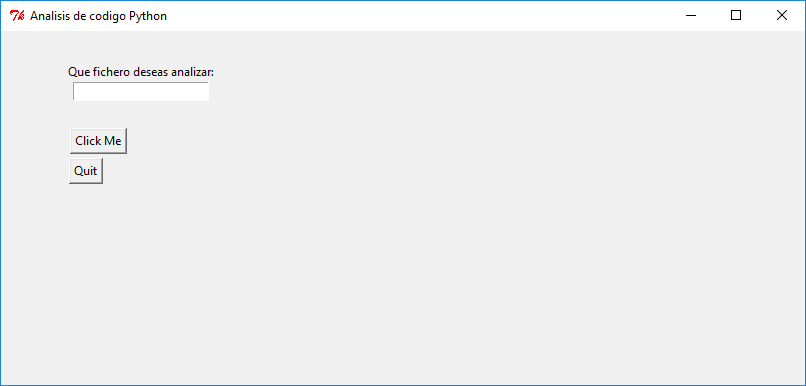
\includegraphics[width=7cm, height=5cm]{VentanaPrincipalOP}
\caption{Ventana principal V.1 Interfaz}
\end{figure}

Para evitar que los elementos colisionasen entre ellos , se pasó a otro  método donde cada vez que se se activasen algunos botones en particular, se añadiese una nueva ventana, esto  evitaba el problema de las colisiones, pero por otra parte la final de los análisis era muy molesto, porque  podías terminar con 4 ventanas diferentes abiertas, lo que al final era muy lioso.\\

\begin{figure}[H]
\centering
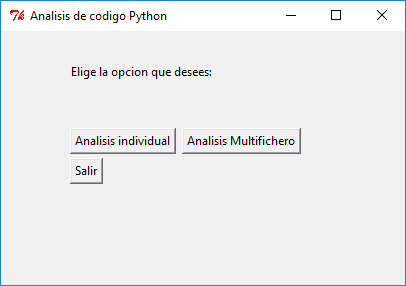
\includegraphics[width=7cm, height=5cm]{VentanaPrincipalOP2}
\caption{Ventana principal V.2 Interfaz}
\end{figure}


Para evitar los problemas tanto de la primera versión de la interfaz como de la segunda, se investigó mas el funcionamiento de la biblioteca Tkinter y sus diferentes funcionalidades, y de esta manera se consiguió realizar una interfaz que utilizase solo una ventana\cite{VideoTkinter2}, pero el contenido  de esta se  fuese cambiando según interactuemos con esta. A decir verdad la interfaz por dentro crea un numero de  marcos, por así llamarlos, donde ya están todos los elementos que se tiene que mostrar en pantalla, cada marco representa un tipo distinto de ventana que puede surgir según se desarrolle la interacción con la herramienta, lo único que solo se muestran por pantalla aquel marco que corresponda con la funcionalidad que se este mostrando en ese momento.\\

Fotos\\

En concreto esta herramienta cuenta con un total de 9 Marcos que son los siguientes:\\

\begin{itemize}
	\item VentanaPrincipal
	\item VentanaIndividual
	\item VentanaAnalisis
	\item VentanaMultiple
	\item VentanaComparacion
	\item VentanaComparacion2
	\item VentanaOperaciones
	\item VentanaOperaciones2
	\item VentanaOperaciones3
\end{itemize}



Es una manera muy útil de hacer una interfaz mucho mas fluida y sencilla para la vista. La única pega que se le podría poner a este método, es que al iniciar la aplicación tiene que generar los marcos para ir rotando entre ellos. Esto ha condicionado más de una vez algunas implementaciones hechas en la interfaz ya que a veces quedan huecos innecesarios.\\

\begin{figure}[H]
\centering
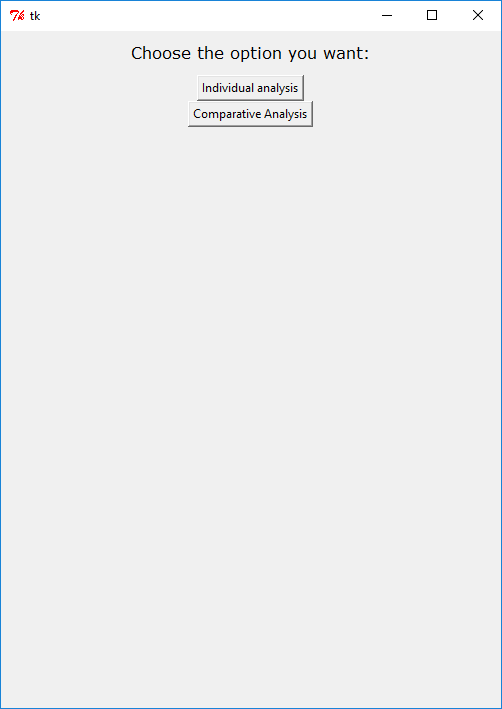
\includegraphics[width=5cm, height=8cm]{VentanaPrincipalExpandido}
\caption{Ventana principal V.3 desconfigurada}
\end{figure}


Para acabar con el desarrollo de las funcionalidades principales se crearon los llamados procesadores teóricos a través de la matriz de traducción. Como ya se ha explicado en puntos anteriores los procesadores contienen una matriz de traducción que contiene valores que dan un nivel de eficiencia a los distintos tipos de operaciones. Para guardar la matriz se decidió utilizar el formato csv. Hay un par de motivos detrás de esta elección:\\

\begin{enumerate}
	\item La simplicidad del formato hace posible poder configurarlo con un gran número de aplicaciones, aunque en el caso de este proyecto se optó por Microsoft Excel.
	\item Hay un modulo de Python en el que ya teníamos algo de experiencia, llamado también csv, que permitía leer y escribir en los tipos de archivos .csv.
\end{enumerate}



\subsection{Artículo}

Una vez terminado el desarrollo de las funcionalidades principales se le dieron unas pinceladas a algunos aspectos de este como proporciones de algunos  elementos en la interfaz, cambios en las nomenclaturas de variables, etc. Y mientras esto ocurría empezamos a desarrollar un artículo sobre el propio proyecto, para exponerlo en el congreso europeo, EuroSim 2019. Pensamos que sería una oportunidad muy buena de ver si el trabajo hecho hasta el momento era visto atractivo y útil por otras personas interesadas en el sector informático y de esta manera también poder aprender del feedback que nos transmitieran.

\subsection{Retoques}
Una vez terminado el artículo se pasó a una fase final de depuración donde se hicieron algunos cambios de diseño o alguna pequeña funcionalidad de última hora. Como por ejemplo cambiar la forma en la que se mostraban los checkboxes\cite{Checkbo}\cite{checkbox} o la parametrización a través del nombre de algunos ficheros.

\section{Estructura interna}


\begin{figure}[H]
\centering
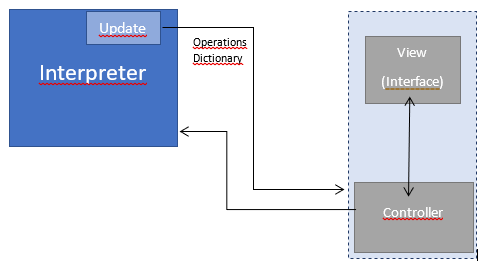
\includegraphics[width=8cm, height=5cm]{Estructura}
\caption{Estructura interna de la herramienta}
\end{figure}

La estructura interna del programa se muestra en la figura 4. Como se puede observar en la figura 4, es un modelo vista controlador . En este caso, el controlador y la vista se implementan de tal manera que comparten algunos componentes, por lo tanto, comparten un cuadro en la imagen, pero aún así, el concepto del modelo es el típico en el que el controlador actúa como un intermediario. Esta unión surgió del desarrollo, se fueron haciendo partes del controlador junto con la interfaz.

En la herramienta, el controlador actúa como un intermediario entre la interfaz gráfica y el interprete. La interfaz permite interactuar y mostrar los resultados del análisis de eficiencia, mientras que el intérprete, el ByteRun en este caso, se ocupa de analizar y ejecutar el código.